\chapter[Historical Context: The Rise and Fall of the Aral Sea]{Historical Context:\\The Rise and Fall of the Aral Sea}
\label{cp:history}

The Aral Sea, once one of the largest inland bodies of water in the world, was a defining geographical feature of Central Asia. By 1960, it spanned approximately 68,000 $km^{2}$, making it the fourth-largest lake globally \cite{britannica_aral}. Fed primarily by the Amu Darya and Syr Darya rivers, it straddled the borders of Kazakhstan and Uzbekistan as seen in \autoref{fig:aral-lake}. The name originates from the Kyrgyz term \textit{Aral-denghiz}, meaning \textit{`Sea of Islands'}, referring to the presence of over 1,000 islands, each exceeding one hectare \textit{(2.5 acres)} in area \autocite{britannica_aral}. For centuries, the Aral Sea supported a rich ecosystem, providing crucial resources such as fresh water, fish, and a stable climate for the surrounding agricultural communities. The lake’s waters served as a vital lifeline for the local population, enabling sustainable fishing industries and agriculture.

\begin{figure}[htpb]
    \centering
    \fbox{\includegraphics[width=0.7\linewidth]{Figures/Aral Lake.png}}
    \caption{Geography of the Aral Lake}
    \label{fig:aral-lake}
\end{figure}

However, the Aral Sea’s decline began in the mid-20$^{th}$ century, driven largely by human intervention. \autoref{fig:satellite-img} illustrates the rapid shrinking of the Aral Lake through satellite images. The most significant factor contributing to its desiccation was the Soviet Union’s aggressive irrigation policies, which diverted vast amounts of water from the two primary rivers that fed the lake to support agricultural expansion \autocite{trushin_aral}. By the early 2000s, the Aral Sea had shrunk by approximately 90\% in volume, leading to a dramatic loss of biodiversity and a collapse of the local fishing industry \autocite{micklin_past}. What was once a thriving body of water became a symbol of ecological devastation. The Aral Sea's loss highlights the complex interplay between industrial development, resource mismanagement, and environmental sustainability. \autoref{cp:aral-now} depicts the current state of the Aral lake.

\begin{figure}
    \centering
    \fbox{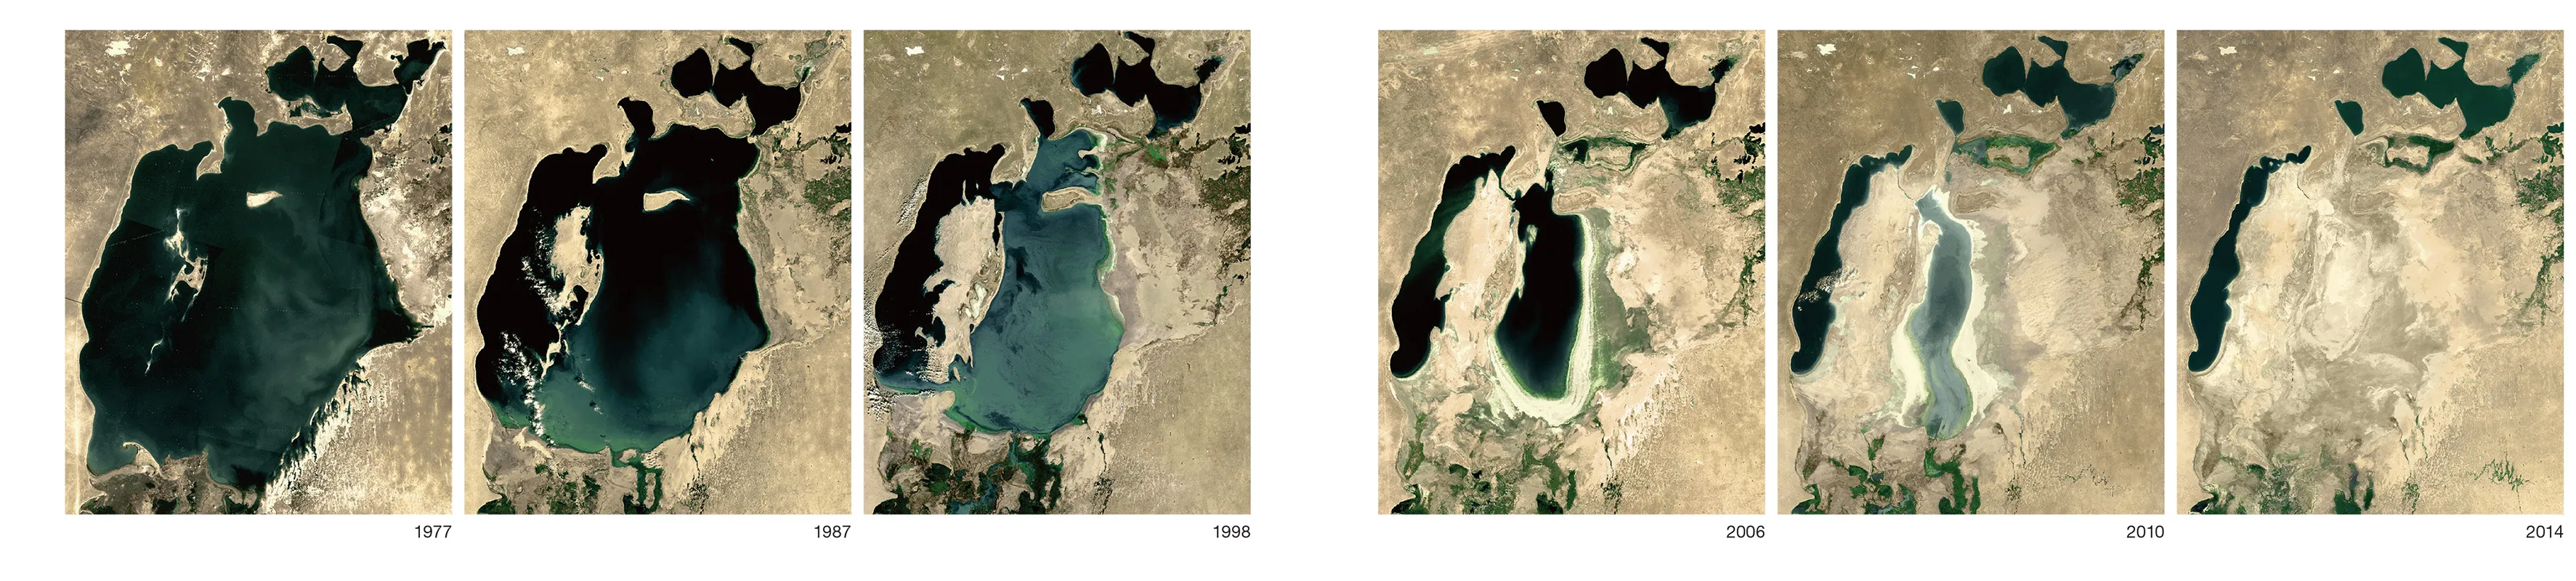
\includegraphics[width=\linewidth]{Figures/Satellite images.png}}
    \caption{Satellite images of the Aral Lake over the years}
    \label{fig:satellite-img}
\end{figure}